\chapter{Methodology}
\justifying

This chapter describes the research design, the dataset and its preparation, the four detection approaches, the training configuration and the evaluation protocol.

\section{Research Design}

The study is an empirical, comparative experiment. All four approaches classify each comment as \emph{toxic} or \emph{non-toxic}, and all are scored on exactly the same held-out test set. Figure~\ref{fig:pipeline} summarises the pipeline.

\begin{figure}[!htb]
  \centering
  \resizebox{\textwidth}{!}{%
  \begin{tikzpicture}[
      box/.style={draw, rounded corners, align=center, minimum height=1cm, text width=3.1cm, font=\small},
      databox/.style={box, fill=blue!8},
      modelbox/.style={box, fill=orange!12, text width=2.6cm},
      resultbox/.style={box, fill=green!10, text width=11.6cm},
      arrow/.style={-{Stealth[length=2.5mm]}, thick}]
    \node[databox] (raw)   at (0,0)   {Raw dataset\\16,073 comments\\6 toxicity labels};
    \node[databox] (clean) at (4.5,0) {Cleaning and\\binary labels\\15,913 comments};
    \node[databox] (split) at (9,0)   {Stratified split\\(seed 42)};
    \node[databox, text width=4.2cm] (train) at (5.1,-2.0) {Training set: 12,730\\90\% fit / 10\% validation};

    \node[modelbox] (lex) at (0,-4.0)    {Lexicon filter\\(better\_profanity)};
    \node[modelbox] (bb)  at (3.4,-4.0)  {BanglaBERT\\fine-tuned};
    \node[modelbox] (xr)  at (6.8,-4.0)  {XLM-RoBERTa\\fine-tuned};
    \node[modelbox] (llm) at (10.2,-4.0) {Zero-shot LLM\\(Qwen via Groq)};

    \node[resultbox] (eval) at (5.1,-5.9) {Evaluation on the same 3,183 test comments:\\accuracy, precision, recall, F1, confusion matrix, speed};

    \draw[arrow] (raw) -- (clean);
    \draw[arrow] (clean) -- (split);
    \draw[arrow] (split.south) |- node[pos=0.25, right, font=\footnotesize] {80\% train} (train.east);
    \draw[arrow] (bb.north |- train.south) -- (bb.north);
    \draw[arrow] (xr.north |- train.south) -- (xr.north);
    \draw[arrow, dashed] (split.east) -- ++(1.4,0) |- node[pos=0.25, right, font=\footnotesize] {20\% test} (eval.east);
    \foreach \m in {lex,bb,xr,llm} \draw[arrow] (\m.south) -- (\m.south |- eval.north);
  \end{tikzpicture}}
  \caption{Experimental pipeline. Only the two fine-tuned models use the training set. The lexicon filter and the LLM need no training. All four approaches are scored on the same held-out test set (dashed arrow).}
  \label{fig:pipeline}
\end{figure}

\section{Dataset}

The experiments use the \textbf{Multi-labeled Bengali Toxic Comments} dataset of Belal et al. \cite{belal2023toxic}, collected from Bangla social media. It contains 16,073 comments. Each comment carries six binary labels; Table~\ref{tab:rawlabels} shows how often each label occurs. A comment can carry several labels at once, and comments with no label are non-toxic.

\begin{table}[H]
  \centering
  \caption{Occurrences of each toxicity label in the raw dataset (16,073 comments). A comment can carry more than one label.}
  \label{tab:rawlabels}
  \begin{tabular}{lrl}
    \toprule
    \textbf{Label} & \textbf{Comments} & \textbf{Description} \\
    \midrule
    Insult    & 2,719 & Insulting or demeaning a person \\
    Vulgar    & 2,505 & Obscene or sexually explicit language \\
    Hate      & 1,898 & Hatred towards a person or group \\
    Troll     & 1,643 & Mocking or provocative trolling \\
    Threat    & 1,419 & Threats of violence or harm \\
    Religious & 1,418 & Attacks on religion or religious groups \\
    \bottomrule
  \end{tabular}
\end{table}

\section{Preprocessing and Label Construction}

The data was prepared with a small conversion script in the following steps:

\begin{enumerate}
  \item \textbf{Binary labelling.} A comment is labelled \emph{toxic} (1) if \emph{any} of the six labels is set, and \emph{non-toxic} (0) otherwise. This turns the task into binary classification, which matches the typical moderation decision of whether to flag a comment.
  \item \textbf{Cleaning.} Leading and trailing whitespace was removed, and empty comments were dropped.
  \item \textbf{De-duplication.} Exact duplicate comments were removed, keeping the first occurrence. This prevents the same text from appearing in both the training and test sets, which would inflate the scores.
\end{enumerate}

No further normalisation, such as stemming or stop-word removal, was applied. The transformer models use their own subword tokenisers, which work best on raw text.

After preprocessing, 15,913 comments remain: 8,459 toxic (53.2\%) and 7,454 non-toxic (46.8\%), so the two classes are reasonably balanced (Figure~\ref{fig:classdist}). Comments are short. They contain 14.3 words (80 characters) on average, the median is 11 words, and the longest comment has 238 words. Figure~\ref{fig:lengths} shows that toxic and non-toxic comments have very similar length distributions, so comment length alone gives little clue to the label.

\begin{figure}[H]
  \centering
  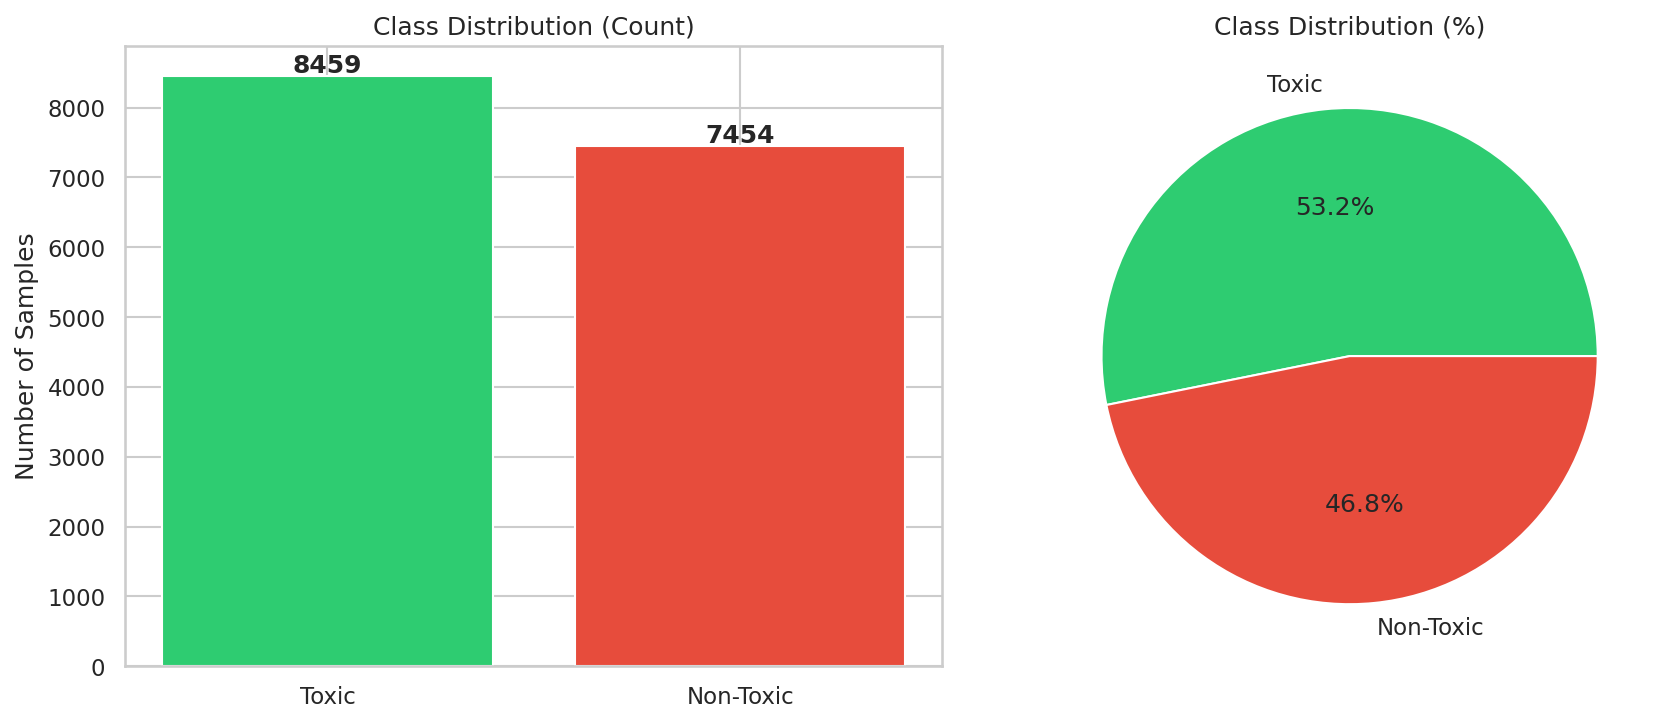
\includegraphics[width=0.9\textwidth]{class_distribution.png}
  \caption{Class distribution after preprocessing (15,913 comments).}
  \label{fig:classdist}
\end{figure}

\begin{figure}[H]
  \centering
  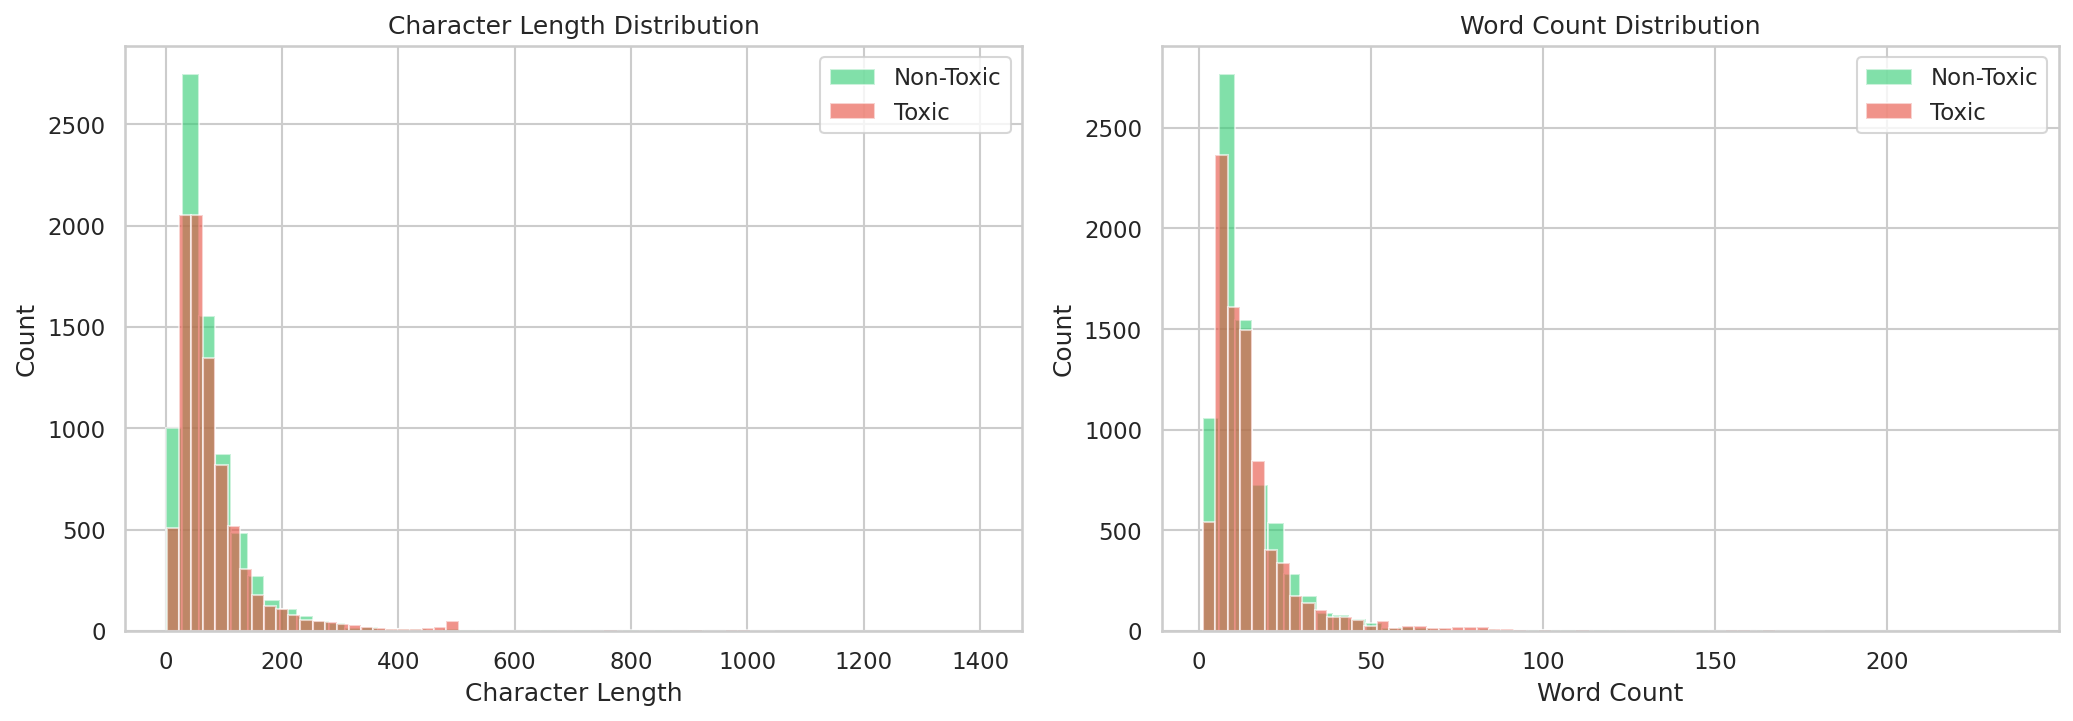
\includegraphics[width=\textwidth]{text_length_distribution.png}
  \caption{Distribution of comment length in characters (left) and words (right) for each class.}
  \label{fig:lengths}
\end{figure}

\section{Data Splitting}

The data was split once with a fixed random seed (42) and stratification by label, so each subset keeps the overall class ratio:

\begin{itemize}
  \item \textbf{Training set:} 12,730 comments (80\%), of which 6,767 are toxic.
  \item \textbf{Test set:} 3,183 comments (20\%), of which 1,692 are toxic and 1,491 non-toxic.
\end{itemize}

For the fine-tuned models, 10\% of the training set (1,273 comments) was further held out as a stratified \textbf{validation set}, leaving 11,457 comments for gradient updates. The validation set is used for early stopping and for choosing the best checkpoint. The test set is used \emph{only} once, to compute the final scores. This avoids a common source of over-optimistic results, where the test set is also used to choose the model. All four approaches are evaluated on the same 3,183 test comments.

\section{Detection Approaches}

\subsection{Lexicon Baseline}

The first baseline is \texttt{better\_profanity} \cite{betterprofanity}, a widely used Python library that flags text containing any word from its built-in profanity list, including common obfuscated spellings. It needs no training. Its list is in English, so it represents the common practice of applying an off-the-shelf filter to a new language without adapting it.

\subsection{BanglaBERT}

BanglaBERT (\texttt{sagorsarker/bangla-bert-base}) \cite{sarker2020banglabert} uses the BERT-base architecture (12 layers, hidden size 768) and was pretrained with masked language modelling on Bangla text only. A linear classification layer is added on top of the \texttt{[CLS]} token representation, and the whole network is fine-tuned on the training data.

\subsection{XLM-RoBERTa}

XLM-RoBERTa (\texttt{xlm-roberta-base}) \cite{conneau2020xlmr} is a multilingual RoBERTa model (12 layers, hidden size 768, about 270 million parameters, most of them in its large 250,000-token vocabulary) pretrained on 2.5 TB of web text in 100 languages. It is fine-tuned in the same way and with the same hyperparameters as BanglaBERT, so the comparison isolates the effect of the pretrained model.

\subsection{Zero-shot Large Language Model}

The LLM baseline uses Qwen (\texttt{qwen/qwen3.8-27b}) \cite{yang2025qwen3}, an open-weight model accessed through the Groq inference API \cite{groqdocs}. The model receives no training examples. Comments are sent in batches of 25, with a fixed instruction asking for one label per comment. Decoding is deterministic (temperature 0), and the model's step-by-step reasoning mode is turned off, so that it returns only the list of labels. A reply is accepted only if it contains exactly one valid label for every comment in the batch; otherwise the batch is retried up to three times.

\section{Training Configuration}

Both transformer models were fine-tuned with the Hugging Face Transformers library \cite{wolf2020transformers} using the settings in Table~\ref{tab:hyper}. They are standard values recommended for fine-tuning BERT-style models \cite{devlin2019bert} and were not tuned further, so that both models are compared under identical conditions.

\begin{table}[H]
  \centering
  \caption{Fine-tuning hyperparameters (identical for both models).}
  \label{tab:hyper}
  \begin{tabular}{ll}
    \toprule
    \textbf{Setting} & \textbf{Value} \\
    \midrule
    Maximum sequence length & 256 tokens \\
    Batch size & 16 \\
    Optimiser & AdamW \\
    Learning rate & $2\times10^{-5}$, linear decay \\
    Warm-up & 10\% of training steps \\
    Weight decay & 0.01 \\
    Maximum epochs & 5 \\
    Early stopping & patience of 2 epochs on validation F1 \\
    Checkpoint selection & best validation F1 (weighted) \\
    Precision & mixed (FP16) \\
    Random seeds & 43, 44, 45 (one per run) \\
    Hardware & NVIDIA T4 GPU (16 GB), Google Colab \\
    \bottomrule
  \end{tabular}
\end{table}

\section{Evaluation Protocol}

\subsection{Metrics}

Predictions are compared with the true labels using accuracy, precision, recall and F1-score. Precision, recall and F1 are averaged over the two classes, with each class weighted by its number of test comments (weighted average). The weighted F1-score is the main metric. Per-class scores, the confusion matrix and the number of false positives (non-toxic comments wrongly flagged) and false negatives (toxic comments missed) are also reported, because the two error types have different costs in moderation.

\subsection{Repeated Runs}

Fine-tuning results vary with the random seed, which controls classifier initialisation and the order of the training data. Each transformer model was therefore trained three times with different seeds, keeping the data splits fixed, and the mean and standard deviation over the three runs are reported. The model from the first run is used for the detailed analysis, such as the confusion matrices, and for the demo.

\subsection{Learning Curve}

To answer RQ5, each transformer model was also trained on the first 25\%, 50\% and 100\% of the (shuffled) training set and evaluated on the full test set.

\subsection{Inference Speed}

Speed is reported as the number of test comments classified per second. For the fine-tuned models, this is measured on the Colab T4 GPU. For the LLM, it includes network round-trips and the pauses required by the free-tier rate limits, so it reflects the practical throughput of this setup rather than the raw speed of the model.

\section{Implementation}

The pipeline is implemented in Python using PyTorch, Hugging Face Transformers \cite{wolf2020transformers} and scikit-learn \cite{pedregosa2011sklearn}. It is organised as six Jupyter notebooks (data exploration, the lexicon baseline, BanglaBERT, XLM-RoBERTa, the LLM baseline, and evaluation), backed by a tested Python package and a command-line entry point. All experiments ran on the free tier of Google Colab. Results are stored on Google Drive, and finished runs are detected and skipped automatically, so an interrupted session can resume without repeating work. A web demo built with Gradio lets a user type a Bangla comment and see the predicted label and confidence.
